\section{Deriving stochastic samplers}
\label{sec:sampling}

\begin{figure}[t]
\centering
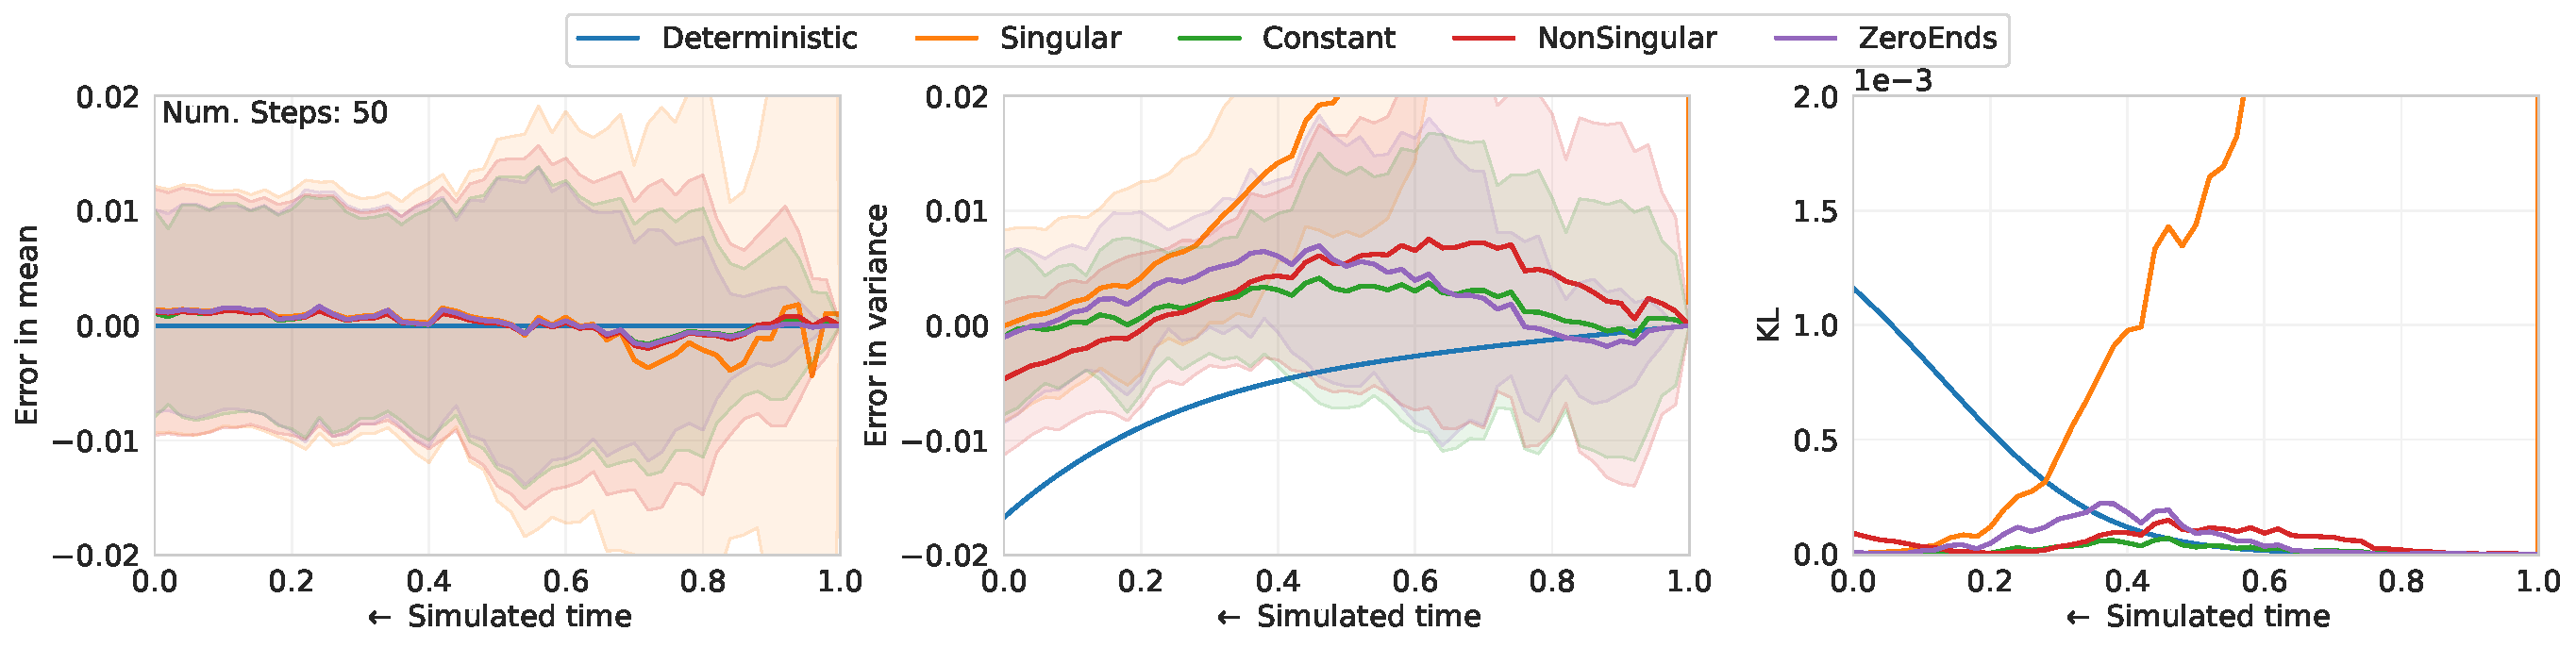
\includegraphics[width=0.99\textwidth]{figs/toy_sampler_comparison_leg_50_kl_2.pdf}
\caption{%
    \textbf{Discretization of deterministic flow leads to bias.}
    Comparison of samplers from \cref{tab:sde_family_table} on the two Gaussian toy problem (\cref{sec:toy_details}).
    Deterministic underestimates the variance parameter, but the stochastic samplers avoid that issue, in exchange for variance in the parameter estimation.
    Singular's variance diverges if we start from $t=1$, so instead we start the sampler at $t=1-10^{-3}$, which allows it to eventually converge by $t=0$.
}
\label{fig:toy_samplers}
\end{figure}

\paragraph{Method intuition.}
Probability flow ODEs \citep{song2020score}, proposed in the context of diffusion models, provide a deterministic sampling method for diffusion models.
These ODEs have the same marginal distribution $p_t(x)$ at all $t$ as the original SDE from which they are derived.
Here, we take the reverse path: we start from an ODE (corresponding to the Gaussian flow model) and deduce the family of SDEs that have the same marginal distributions at all $t$ as the original ODE.
Before we introduce the general result, we will show a naive approach that gives an SDE with a problematic singularity, motivating the need for the generalization.

%%%%%%%%%%%%%%%%%%%%%%%%%%%%%%%%%%%%%%%%%%%%%%%%%%%%%%%%%%%%%%%%%%%%%
\subsection{A singular SDE corresponding to Gaussian flow}
\label{sec:gaussian_flow_sde}

For Gaussian flow, $p_1(x_1)\equiv N(x_1; \mu_1, \sigma_1^2I)$ is assumed to be Gaussian.
With interpolation $x_t = (1-t)x_0 + tx_1$, the perturbation kernel $p(x_t | x_0) = N(x_t; (1-t)x_0+t\mu_1, t^2\sigma_1^2I)$ is also Gaussian.

Note that since $x_0, x_1$ are independent, we can directly infer the first and second moments $\mu_t, \Sigma_t$ for the marginals $p_t(x)$ as $\mu_t =  (1-t)\mu_0 + t\mu_1$ and $\Sigma_t = (1-t)^2\Sigma_0 + t^2\sigma_1^2I$.
With these constraints and choosing $\mu_1 \equiv 0, \sigma_1 \equiv 1$, we can solve for drift and diffusion coefficients that yield the same marginal distributions:
\begin{align}
\label{eq:singular_choices}
f(x, t) &= -\frac{x}{1-t} & g(t) &= \sqrt{\frac{2t}{1-t}}
\end{align}
See \cref{sec:singular_sde_app} for the details and a more general expression for arbitrary $\mu_1, \sigma_1$.
The coefficients $f(x, t), g(t)$ are singular at the boundary $t=1$ of the interval.
Consequently, simulation methods such as Euler-Maruyama, that need $f(x, t), g(t)$ to be Lipschitz are not guaranteed to work at the boundary (see \cref{fig:toy_samplers} and \cref{sec:guass_experiments}).
We refer to this SDE as the Singular SDE.
An empirical trick that is often used in such cases is to assume $p_{1-\epsilon}(x_{1-\epsilon}) \approx p_1(x_1),  \epsilon \ll 1$.
However, this can lead to unpredictable behavior and we show how to avoid it in the following section.

%%%%%%%%%%%%%%%%%%%%%%%%%%%%%%%%%%%%%%%%%%%%%%%%%%%%%%%%%%%%%%%%%%%%%
% \subsection{A general form for Gaussian flow SDEs}
\subsection{Set of SDEs that share the same marginal distribution $p_t(x)$}
\label{sec:general_sde}

First we state our general result with the diffusion coefficient $G(x, t)$ a function of both the state $x$ and time $t$, and then state simpler forms more directly applicable to models used in practice.

\begin{restatable}{theorem}{mainresult}
\label{thm:general}
Let $p_t(x)$ be the probability density of the solutions of the SDE in \cref{eq:general_sde_paper}
evolving as $\frac{\partial p_t}{\partial t}$.
Then, the probability density of solutions of the following set of SDEs, indexed by $\GT, \gamma_t$, also evolves as $\frac{\partial p_t}{\partial t}$.
\begin{align}
\label{eq:result_sde}
dx = \bar f(x,t)dt + \bar G(x, t)dW_t
\end{align}
where
\begin{align}
\bar f &= f - \frac{1}{2}\left(\nabla \cdot [(1-\gamma_t)GG^T-\GT\GT^T] + [(1-\gamma_t)GG^T-\GT\GT^T]\cdot\nabla\ln p_t \right)\\
\bar G &= [\gamma_t GG^T + \GT\GT^T]^{\frac{1}{2}}
\end{align}
and $\GT \equiv \GT(x, t), \gamma_t \ge 0$ are arbitrary functions such that the solutions of \cref{eq:result_sde} exist and are unique.
\end{restatable}

Proof of \cref{thm:general} is given in \cref{sec:mainresult_proof_app} and follows from manipulations of Fokker-Planck-Kolmogorov (FPK) equations corresponding to \cref{eq:result_sde}.

\cref{thm:general} implies that given the same initial density $p_0(x)$, evolution according to both \cref{eq:general_sde_paper} and \cref{eq:result_sde} will have the same marginal densities $p_t(x)$ for all times $t$.
Further, \cref{eq:result_sde} can be simulated backward in time using the result from \citet{anderson1982reverse}, again with the same marginal densities $p_t(x)$.
Consequently, \cref{eq:general_sde_paper} can be simulated forward or backward in time using any member of the family specified by \cref{eq:result_sde}.
Note that setting $\gamma_t=1, \GT = 0$ recovers the original SDE in \cref{eq:general_sde_paper}, while setting $\gamma_t=0,\GT = 0$ recovers the general probability flow ODE from \citet[eq. 37]{song2020score}.
Additionally, $\GT$ is particularly useful for deterministic flow models, further discussed in \cref{cor:detflow_corollary}.
\cref{thm:general} gives a recipe for developing particular samplers, such as those in the remainder of this section, some of which have appeared in the literature.
A priori, \cref{thm:general} cannot determine which concrete sampler will be best for a given application, but since the samplers do not require any training to use, it is possible to postpone the choice of sampler to an empirical analysis at test time.

The flexibility afforded by \cref{eq:result_sde} is particularly useful
\textbf{(1)} in the presence of singularities in the drift and diffusion coefficients $f$ and $G$ respectively of \cref{eq:general_sde_paper},
\textbf{(2)} in the presence of errors resulting from finite discretization,
and \textbf{(3)} for flexible specification of the diffusion coefficient in generative applications.
Our experimental evaluations primarily focus on these aspects of \cref{thm:general}.

A direct consequence of \cref{thm:general}, by defining $\GT\equiv0, G \equiv g(t)I$, is the following corollary applicable to commonly used generative diffusion models with additive noise:
\begin{restatable}{corollary}{corollaryone}
\label{cor:diffusion_corollary}
For the SDE in \cref{eq:general_sde_paper} with $G\equiv g(t)I$, a subset of SDEs prescribed by \cref{thm:general} and indexed by $\gamma_t$ is:
\begin{align}
dx &= \left[f(x, t) - \frac{(1 - \gamma(t))g^2(t)}{2}\nabla_x \ln p_t(x)\right]dt + \sqrt{\gamma(t)} g(t) dW_t
\label{eq:diffusion_corollary}
\end{align}
\end{restatable}
Proof in \cref{sec:corollaryone_proof_app}.
Note that choosing $\gamma_t = 0$ results in the probability flow ODE specified in \cref{eq:probflow_ode_song}.
Intuitively, the members in the family differ in terms of the amount of noise injected as a function of time.
$\gamma_t = 0$ yields a purely deterministic simulation; $\gamma_t > 0$ yields a variety of stochastic simulations.
Further, similar special cases discussed in \cite{huang2021variational} and \cite{berner2022optimal} also directly follow from \cref{thm:general} as well.

Some properties of \cref{cor:diffusion_corollary}:
\begin{enumerate}[leftmargin=*]
    \item $\gamma(t)$ can be chosen at sampling time and doesn't affect the training of the score function.
    \item With $\gamma(t) = \hat \gamma^2(t)g^{-2}(t)$, where $\hat \gamma(t)$ is an arbitrary function (satisfying constraints of \cref{thm:general}), we can choose an arbitrary diffusion term at sampling time.
    For example, choosing $\gamma_t = \gamma^2/g^2(t)$ leads to a constant diffusion coefficient.
    \item For the SDE specified by \cref{eq:singular_choices}, we can choose $\gamma(t) = (1-t)\hat \gamma^2(t)g^{-2}(t)$ to get rid of the singularity in the diffusion term.
\end{enumerate}

Note that \cref{thm:general} can be used whenever we have access to the score function $\nabla_x \ln p_t$.
Next, we first construct a specialized solution based on \cref{thm:general} for deterministic flow models that enables flexible control of both drift and diffusion coefficients, and apply it to the special case of deterministic Gaussian flows where the score function can be imputed from the velocity field (\cref{sec:score_function}).
Recall that deterministic flows specify a transport via the ODE $dx = v(x, t)dt$.
This ODE can be viewed as an SDE where the diffusion term has been set to zero.
Choosing $G \equiv 0, \GT \equiv \tilde g(t)I$ in \cref{thm:general} gives \cref{cor:detflow_corollary}, which enables deriving stochastic samplers for Gaussian flow models:
\begin{restatable}{corollary}{corollarytwo}
\label{cor:detflow_corollary}
For the ODE in \cref{eq:rect_flow_ode}, a subset of SDEs prescribed by \cref{thm:general} and indexed by $\tilde g(t)$ is
\begin{align}
\label{eq:detflow_corollary}
dx &= \left[v(x, t) + \frac{\tilde g^2(t)}{2}\nabla_x \ln p_t(x)\right]dt + \tilde g(t) dW_t
\end{align}
\end{restatable}
Proof in \cref{sec:corollarytwo_proof_app}.
\cref{cor:detflow_corollary} enables flexible specification of a time dependent diffusion coefficient $\tilde g(t)$, allowing the introduction of stochasticity in the simulation of otherwise deterministic models, \emph{purely at sampling time}.
Note that \cref{eq:detflow_corollary} requires access to the score function $\nabla_x \ln p_t(x)$ for the marginal distributions $p_t(x)$.  In \cref{sec:score_function}, we describe how the score function can be imputed from the learned flow model $v(x, t)$ for the special case of Gaussian flow models.
It can be verified that the particular choice of $f$ and $g$ in \cref{eq:singular_choices}  satisfy \cref{eq:detflow_corollary} by using the expression for the score from \cref{eq:rect_score}.

\begin{table}[t]
  \caption{%
    Examples of SDEs that have the same marginal distribution $p_t(x)$ as a given Gaussian flow specified by $v\equiv v(x,t)$.
    $\alpha \ge 0$ is a scale parameter that varies the magnitude of the diffusion coefficient $g$.
    Each of these behaves differently when discretized and simulated (\Cref{fig:toy_samplers} and \cref{sec:diff_coeff_mag_qual}).
    These and infinitely many more can be constructed using the scheme in \cref{eq:detflow_corollary}.
  }
  \label{tab:sde_family_table}
  \centering
  \begin{tabular}{lLLl}
    \toprule
    Name &\tilde g(t) & \tilde f(x, t) &  Description  \\
    \midrule
    Deterministic &  0 & v & Base flow model  \\
    Constant & \alpha & v + \frac{\alpha^2}{2} \nabla_x \ln p_t & \text{Constant $g$, singular $f$} \\
    Singular & \alpha \sqrt{t/(1-t)} & v + \frac{\alpha^2}{2}\frac{t}{1-t} \nabla_x \ln p_t  & Singular $g, f$\\
    NonSingular & \alpha\sqrt{t}, & v + \frac{\alpha^2}{2}t\nabla_x \ln p_t & \text{Non-singular} $g,f$ \\
    ZeroEnds & \alpha\sqrt{t(1-t)}, & v + \frac{\alpha^2}{2}t(1-t)\nabla_x \ln p_t & Non-singular $g,f, g(0)=g(1)=0$ \\
    \bottomrule
  \end{tabular}
\end{table}

While infinitely many choices are available for $\tilde g$, we consider a few interesting ones listed in the \cref{tab:sde_family_table}, constructed by choosing integer powers of $t$ and $1-t$ and introducing a scaling coefficient $\alpha$, for experimental evaluations.
Note that the only degree of freedom in \cref{tab:sde_family_table} is the choice of $\tilde g(t)$, which determines $\tilde f(x, t)$, given the flow field $v(x, t)$ and the score $\nabla_{x}\ln p_t(x)$.
The $f(x,t)$ is singular in Constant because the score $\nabla_x \ln p_t(x_t)$, as computed in \cref{eq:rect_score}, has $t$ in the denominator, making $f(x, t)$ singular at $t=0$.
The choice in NonSingular precisely eliminates this singularity.
\Cref{fig:toy_samplers} compares these choices in a toy setup; \cref{sec:experiments} has comparisons on ImageNet.

%%%%%%%%%%%%%%%%%%%%%%%%%%%%%%%%%%%%%%%%%%%%%%%%%%%%%%%%%%%%%%%%%%%%%
\subsection{Score function and classifier free guidance for a Gaussian flow model}
\label{sec:score_function}

Recall that \cref{thm:general} requires access to the score function.
For Gaussian flows, the score function can be inferred from the velocity field itself, alleviating the need to learn it separately.
This result is known (see e.g. \cite{zheng2023guided} in the context of flow matching) and we present it here in our setting.
For Gaussian flows, with $p_1(x_1) \equiv N(x_1; \mu_1, \sigma_1^2I)$ and interpolation specified in \cref{eq:rect_flow_default_interp}, the score can be computed as:
\begin{align}
\label{eq:rect_score}
\nabla_{x} \ln p_t(x) &= \frac{-(1-t)v(x, t)+\mu_1-x}{t\sigma_1^2}
\end{align}
where $v(x, t) = \E [x_1-x_0 | x, t]$ is the estimated flow.
Proof is provided in \cref{sec:score_fn_app}.
Note that the score function can also be estimated given $\E [x_0 | x, t]$ or $\E [x_1 | x, t]$.
In summary, the expression follows directly from using results from Denoising Score Matching \citep{vincent2011connection} and the Gaussianity of $p_1(x_1)$.
Similar expressions can be derived for other interpolations that are linear in $x_0, x_1$.
With access to the score function and linearity of \cref{eq:rect_score} in $v$ we can define classifier free guided~\citep{ho2022classifier} Gaussian flow as:
\begin{align}
v_{\text{cfg}}(x, t, c) = (1 + \lambda)v(x, t, c) - \lambda (v(x, t, c=\varnothing)
\end{align}
where $c$ indicates extra conditioning information as in classifier free guidance, $\varnothing$ indicates no conditioning and $\lambda$ specifies the relative strength of the guidance.
$\lambda = 0$ reduces to class conditional sampling, while $\lambda > 0$ puts a larger weight on the conditioning, biasing the sample towards the modes of the conditional distribution.
Using classifier-free guidance with a stochastic sampler will, of course, give diversity that isn't possible with a deterministic sampler, as can be seen in \cref{fig:imagenet_cfg}.
Note that \cite{xie2024reflected,dao2023flow,zheng2023guided} also consider related definitions in the context of flow matching.

